\documentclass[11pt,a4paper]{article}

\usepackage[T1]{fontenc}
\usepackage[utf8]{inputenc}
\usepackage{mathptmx}
\usepackage{courier}
\usepackage[margin=2.5cm]{geometry}
\usepackage{amsmath}
\usepackage{booktabs}
\usepackage{graphicx}
\usepackage{xcolor}
\usepackage[numbers,sort&compress]{natbib}
\usepackage{xurl}
\usepackage[hidelinks]{hyperref}
\hypersetup{pdftitle={When Splitting Hurts: Task Decomposition for Small Local LLMs Filling Clinic Forms in English and Roman Urdu},pdfauthor={Muzammal Hussain and Maryam Khalid}}
\usepackage{caption}
\captionsetup{font=small,labelfont=bf}

\newcommand{\code}[1]{\texttt{#1}}
\setlength{\emergencystretch}{3em}

\title{\textbf{When Splitting Hurts: Task Decomposition for Small Local\\LLMs Filling Clinic Forms in English and Roman Urdu}}
\author{Muzammal Hussain$^{1}$ \qquad Maryam Khalid$^{2}$\\[4pt]
\small $^{1}$Independent researcher, Glasgow, United Kingdom\\
\small $^{2}$Physiotherapist, Glasgow, United Kingdom\\
\small Correspondence: \href{mailto:muzammal@masmatixinnovations.co.uk}{muzammal@masmatixinnovations.co.uk}\\
\small ORCID (M.\ Hussain): \href{https://orcid.org/0009-0001-2570-5686}{0009-0001-2570-5686}}
\date{\small November 2026}

\begin{document}
\maketitle

\begin{abstract}
\noindent
Agent designers often split a task into smaller sub-calls, expecting each to be easier. We test this on a narrow,
controlled case: two small open-weight models (\code{llama3.1:8b} and \code{qwen2.5:3b}) run locally fill an
eight-field physiotherapy-clinic form from a case note in 1, 2, 4 or 8 sub-calls, with notes in English and in Roman
Urdu, and with either independent fields or chained billing fields in which later values are computed from earlier
ones. Across 512 forms and 1,920 sub-calls, with answers merged by code, splitting independent fields cost little:
nothing for English notes and at most 8.6 points of field accuracy for Roman Urdu. Splitting chained fields cost a
great deal: against a single call, \code{llama3.1:8b} lost 35.9 to 47.7 points on English notes (paired 95\%
intervals all below zero) and \code{qwen2.5:3b} lost 18.0 to 43.8. Most of the loss traced to one field. Asked for the
fee per session without the neighbouring billing fields, \code{llama3.1:8b} returned the fee after the discount in 35
of its 36 wrong English values, an error it never made when all fields were requested together; the mistake then
propagated to the gross fee, discount and amount payable. The field description did not say ``before discount'', so
the result shows how splitting removes context that disambiguates a field. Roman Urdu notes lowered accuracy on
extraction (joint, side and weekday) by 15 to 28 points, independently of splitting. Splitting also multiplied
sequential time by about three and prompt length by about five. For small local models filling structured forms,
the default should be one call per form; split only independent fields, and only when parallel speed is needed.
Cases, prompts, raw replies and analysis code are public.
\end{abstract}

\noindent\textbf{Keywords:} LLM agents; task decomposition; structured extraction; local language models; Roman Urdu; clinical documentation

\section{Introduction}

A common design move in LLM agents is to break a task into smaller pieces. Decomposed Prompting assigns sub-tasks
to dedicated prompts~\cite{khot2023decomposed}; ADaPT decomposes recursively when the executor
fails~\cite{prasad2023adapt}; and task-graph systems such as Plan-over-Graph and DynTaskMAS split work so that parts
can run in parallel~\cite{zhang2025plangraph,yu2025dyntaskmas}. The intuition is that a smaller question is easier,
especially for a small model. The cost is less often measured: each sub-call sees less of the task.

This matters for small clinics that want local models to fill structured records from consultation notes, because
patient data should not leave the clinic and local hardware favours models of a few billion
parameters~\cite{qwen2025qwen25,grattafiori2024llama3}. It matters more where staff write in Roman Urdu, which our
earlier work found harder for small local agents~\cite{hussain2026romanurdu}. We therefore hold one task fixed, filling
an eight-field form, and ask:

\begin{enumerate}
  \item How does splitting the form into 1, 2, 4 or 8 sub-calls change field accuracy, whole-form correctness and
  cost?
  \item Does the answer differ between fields that are independent and fields that depend on earlier ones?
  \item Does it differ between English and Roman Urdu notes?
\end{enumerate}

Companion benchmarks measure the repeated-trial reliability of tool calls \cite{hussain2026toolcall} and routing between retrieval agents \cite{hussain2026router}.

\section{Method}

\paragraph{Forms and notes.} Each case is a short physiotherapy note with a form of eight fields. \emph{Independent}
forms ask for the patient's age, the side and joint that hurt, the pain score, sessions per week, number of weeks, the
fee per session and the day of the next review. \emph{Chained} forms ask for billing values in which later fields are
computed from earlier ones: sessions per week, weeks, total sessions (their product), fee per session, gross fee
(total sessions $\times$ fee), discount percent, discount amount and the amount payable. Each field has a one-line
description in the prompt, for example ``fee per session in rupees in the current course, as a number''. Notes also
contain distractors the model must ignore, such as a relative's age or the details of a closed earlier course. There
are 16 independent and 16 chained cases, generated from a fixed seed, each written as an English note and a Roman Urdu
note with the same facts. Instructions and JSON keys stay in English.

\paragraph{Splitting.} At granularity $g \in \{1,2,4,8\}$ the eight fields are cut into $g$ equal consecutive groups
and each group is one model call. Code merges the answers; no model takes part in merging. In chained forms each
sub-call receives the values produced by earlier sub-calls exactly as produced, so an early mistake can reach later
fields. The field list precedes the note in every prompt so that prompt caching does not make later sub-calls look
cheaper.

\paragraph{Models and measures.} \code{llama3.1:8b} and \code{qwen2.5:3b} ran through Ollama 0.40.15 on a MacBook with
temperature 0, seed 42, JSON output mode, a 2,048-token context and at most 256 output tokens. The full grid is 2 models
$\times$ 2 languages $\times$ 2 dependency types $\times$ 4 granularities $\times$ 16 cases = 512 forms and 1,920
sub-calls. We report field accuracy (share of the eight fields correct), all-fields-correct, computed-step accuracy
(for chained forms, how often a computed field is right when its inputs are right), JSON failures, summed seconds and
prompt length. ``Ideal parallel'' time is the slowest sub-call for independent forms and the sum for chained forms; it
is derived from the sequential run, not measured. Intervals are 95\% percentile bootstrap intervals over the 16 cases
(2,000 resamples)~\cite{efron1993bootstrap}; comparisons with one call and between languages are paired on the same
cases.

\paragraph{Clinician review.} After the runs, a physiotherapist (M.K.) read all 32 cases in both languages with the expected form values. She marked every expected value correct and both notes of every case equal in facts. She judged the 16 chained (billing) notes realistic and, in all 16, found ``fee per session'' clear without the discount when the whole note is read. She judged none of the 16 independent notes realistic: every comment names the distractor line about the patient's brother's age and earlier fee, which would not appear in a real physiotherapy note.

\section{Results}

All 512 forms finished and no reply failed to parse. Figure~\ref{fig:acc} and Table~\ref{tab:paired} summarise the
effect of splitting.

\begin{figure}[t]
  \centering
  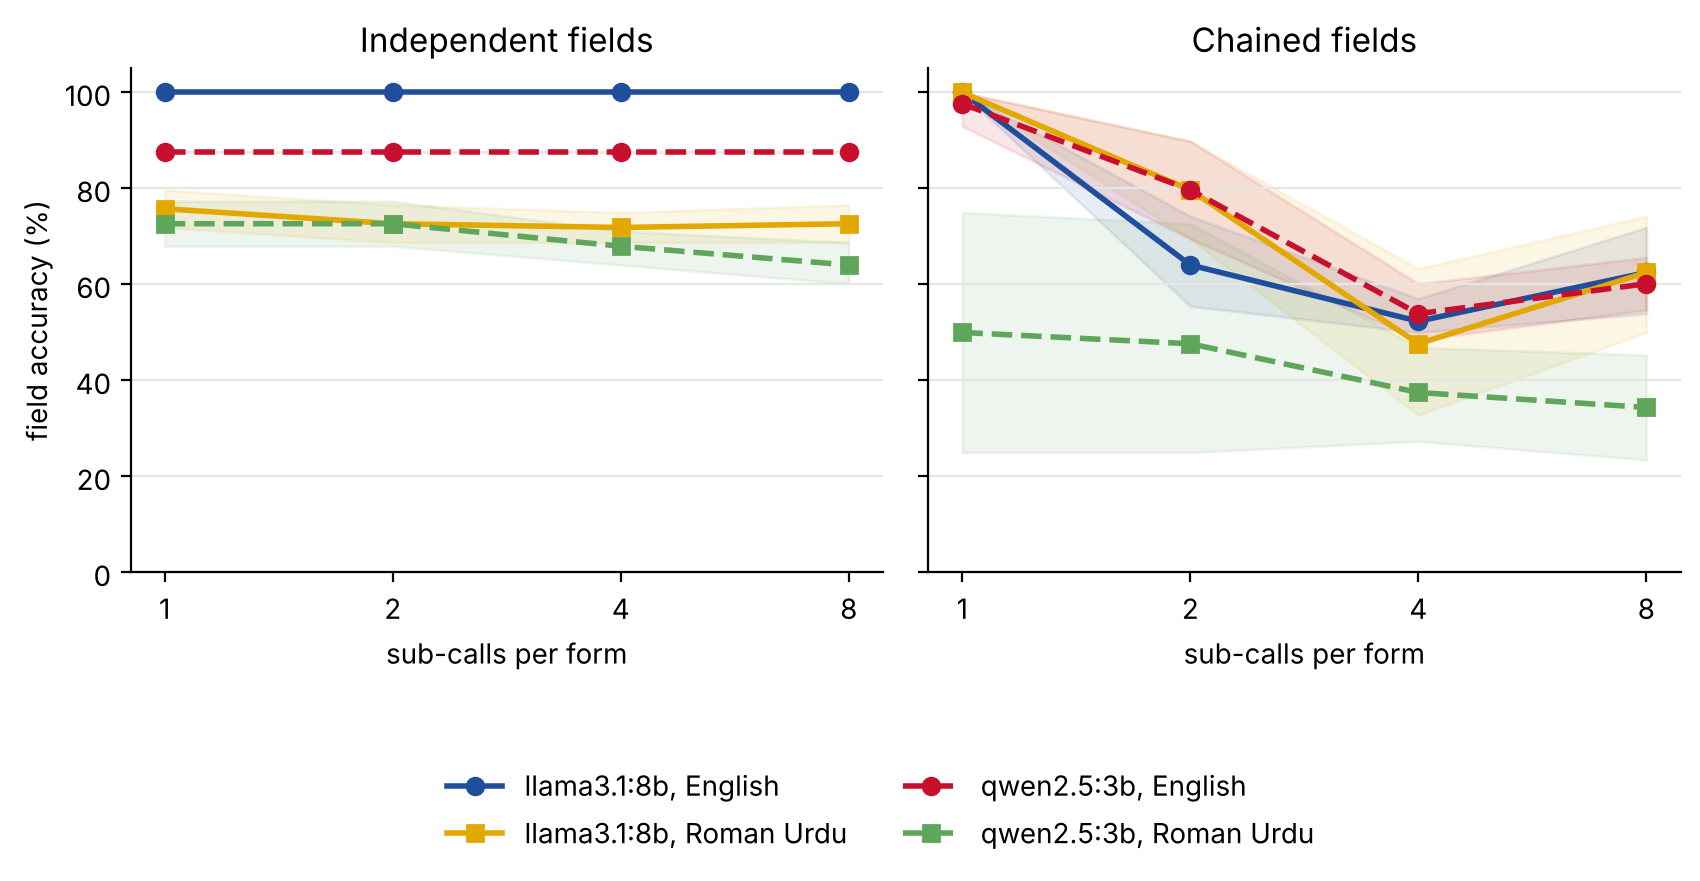
\includegraphics[width=\linewidth]{figures/fig_accuracy.png}
  \caption{Field accuracy against the number of sub-calls per form (16 forms per point; shaded: 95\% bootstrap
  intervals).}
  \label{fig:acc}
\end{figure}

\begin{table}[t]
\centering
\small
\caption{Change in field accuracy against one call (percentage points, paired 95\% bootstrap intervals over 16
cases).}
\label{tab:paired}
\setlength{\tabcolsep}{3.5pt}
\footnotesize
\begin{tabular}{lllccc}
\toprule
Model & Note & Fields & 2 calls & 4 calls & 8 calls \\
\midrule
\code{llama3.1:8b} & English & independent & 0.0 & 0.0 & 0.0 \\
\code{llama3.1:8b} & English & chained & $-35.9$ [$-44.5$, $-25.8$] & $-47.7$ [$-50.0$, $-43.0$] & $-37.5$ [$-46.1$, $-28.1$] \\
\code{llama3.1:8b} & Roman Urdu & independent & $-3.1$ [$-6.2$, $-0.8$] & $-3.9$ [$-7.0$, $-1.6$] & $-3.1$ [$-6.2$, $-0.8$] \\
\code{llama3.1:8b} & Roman Urdu & chained & $-20.3$ [$-30.5$, $-10.2$] & $-52.3$ [$-67.2$, $-36.7$] & $-37.5$ [$-50.0$, $-25.8$] \\
\code{qwen2.5:3b} & English & independent & 0.0 & 0.0 & 0.0 \\
\code{qwen2.5:3b} & English & chained & $-18.0$ [$-28.1$, $-7.8$] & $-43.8$ [$-50.0$, $-36.7$] & $-37.5$ [$-44.5$, $-29.7$] \\
\code{qwen2.5:3b} & Roman Urdu & independent & 0.0 & $-4.7$ [$-12.5$, 2.3] & $-8.6$ [$-16.4$, $-1.6$] \\
\code{qwen2.5:3b} & Roman Urdu & chained & $-2.3$ [$-7.0$, 0.0] & $-12.5$ [$-31.2$, 5.5] & $-15.6$ [$-33.6$, 1.6] \\
\bottomrule
\end{tabular}
\end{table}

\subsection{Independent fields survive splitting}

For English notes, splitting independent fields changed nothing for either model: \code{llama3.1:8b} filled every
field correctly at every granularity, and \code{qwen2.5:3b} stayed at 87.5\%. For Roman Urdu notes the losses were
small: 3.1 to 3.9 points for \code{llama3.1:8b} and up to 8.6 points for \code{qwen2.5:3b} at eight calls.
\code{qwen2.5:3b}'s ceiling of 87.5\% on English independent forms is one field: it wrote weekday abbreviations such as
``tue'' where the description asked for a full lower-case weekday.

\subsection{Chained fields do not}

With all eight billing fields in one call, \code{llama3.1:8b} filled every chained form correctly in both languages,
and \code{qwen2.5:3b} reached 97.7\% field accuracy on English notes. Splitting cost both models heavily. On English
notes \code{llama3.1:8b} fell to 64.1\%, 52.3\% and 62.5\% at 2, 4 and 8 calls, and whole forms were correct in 18.8\%,
0\% and 12.5\% of cases instead of 100\%. \code{qwen2.5:3b} fell to 79.7\%, 53.9\% and 60.2\%, with no fully correct
form at 4 or 8 calls. The losses were not monotonic: four calls was worse than eight for both models in English;
we do not have a tested explanation for this.

\subsection{One field explains most of the loss}

When \code{fee\_per\_session} was requested without the other billing fields, \code{llama3.1:8b} often returned the fee
after the discount: 35 of its 36 wrong English fee values in split forms equal fee $\times$ (100 $-$ discount)/100
(Figure~\ref{fig:fee}). With all fields in one call, where the gross fee and discount are requested alongside, it made
no such error. Because the fee feeds the gross fee, the discount amount and the payable amount, one misread field
became four wrong fields. The arithmetic itself held up for \code{llama3.1:8b}: when the inputs to a computed field were
right, the computed field was right in 86 to 100\% of English cases. \code{qwen2.5:3b} made the discounted-fee error less
often (7 of 17 wrong English fees) but its arithmetic broke down in short sub-calls: computed-step accuracy fell from
98.4\% in one call to 62.5\% and 48.3\% at 4 and 8 calls.

\begin{figure}[t]
  \centering
  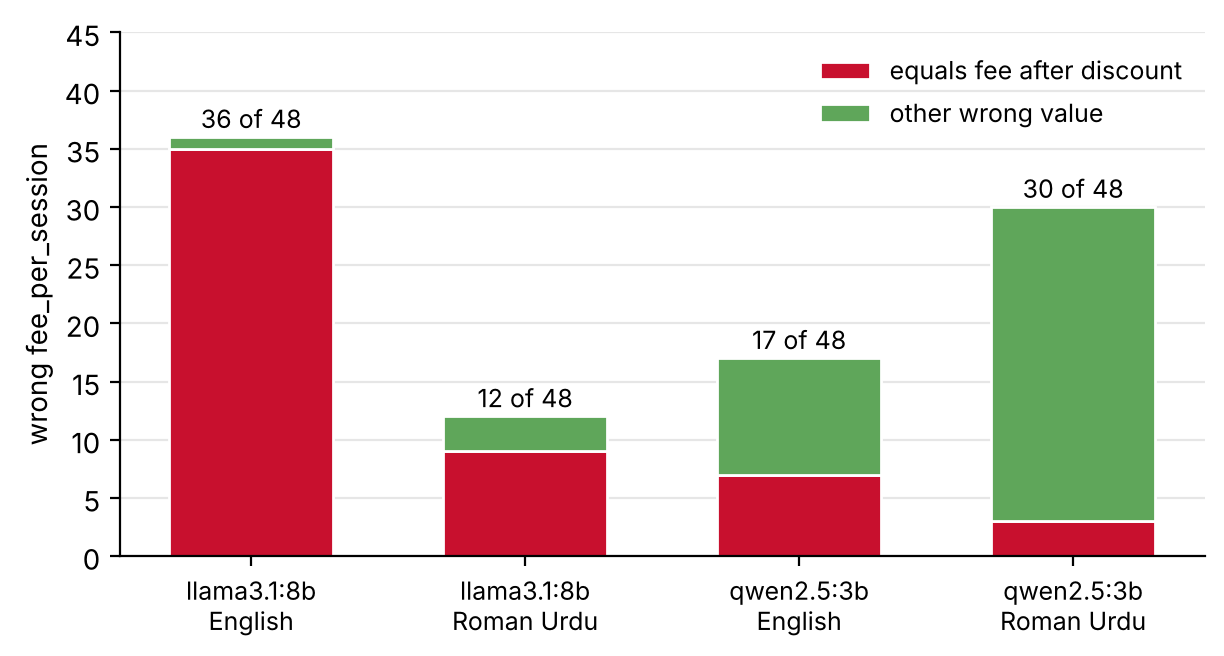
\includegraphics[width=0.72\linewidth]{figures/fig_fee.png}
  \caption{Wrong \code{fee\_per\_session} values in split chained forms (48 per bar: 16 cases $\times$ 3 split
  levels), and how many equal the fee after the discount.}
  \label{fig:fee}
\end{figure}

The field description, ``fee per session in rupees in the current course'', does not say whether the fee is before or
after the discount. A single call settles this implicitly, because the same form also asks for a discount and a gross
fee computed from the fee. A sub-call that sees only the fee loses that context. The result is therefore partly about
an underspecified field and partly about splitting removing the context that disambiguated it; in practice the two go
together, because real form descriptions are rarely complete.

\subsection{Roman Urdu hurts extraction, not splitting}

Roman Urdu notes lowered field accuracy on independent forms by 24.2 to 28.1 points for \code{llama3.1:8b} and by 14.8
to 23.4 points for \code{qwen2.5:3b}, at every granularity. Typical one-call errors were the joint (``knee'' for a hip
or ankle), the side, and the review day left untranslated (for example \emph{mangal} for Tuesday). For chained forms
the picture differed by model: \code{llama3.1:8b} filled every Roman Urdu form in one call and made fewer
discounted-fee errors when split (9 of 48), whereas \code{qwen2.5:3b} reached only 50.0\% field accuracy even in one
call. Splitting and language therefore acted largely separately: Roman Urdu made reading the note harder; splitting
made the billing logic fragile.

\subsection{Cost}

Splitting multiplied the prompt the model had to read, because every sub-call repeats the note. For \code{llama3.1:8b}
on English independent forms, prompt length grew from about 1,100 characters in one call to about 5,600 across eight,
and summed time from 5.9 to 18.5 seconds. If the eight calls ran in parallel the slowest would take 4.2 seconds, a
modest saving over one call. For chained forms there is no parallel saving, because each sub-call waits for the
previous one: eight calls took 24.9 seconds against 7.7 for one.

\section{Discussion}

\paragraph{Default to one call per form.} For an eight-field form, one call was as good as or better than any split in
every condition we tested, and much better whenever fields depended on each other. Splitting independent fields was
nearly harmless but bought speed only with parallel hardware, which a single clinic computer may not have.

\paragraph{Splitting removes disambiguating context.} The discounted-fee error shows the mechanism. Fields on a form
explain each other: asking for a discount and a gross fee alongside the fee tells the model which fee is meant. A
sub-call that sees one field inherits none of that. Decomposition frameworks usually assume sub-tasks are
self-contained; for extraction from notes they rarely are. This fits the clinician review: reading the whole note, our reviewer found ``fee per session'' clear in all 16 chained notes.

\paragraph{If you split, compute in code.} The chained fields here are arithmetic on extracted values. Once the model
has extracted sessions, weeks, fee and discount, code can compute the rest exactly. This avoids both the propagation of
early mistakes and \code{qwen2.5:3b}'s arithmetic errors in short sub-calls, and it reduces the model's job to the part
only a model can do.

\paragraph{Write complete field descriptions.} A field that is clear inside a full form can be ambiguous on its own.
When fields are split, each description should carry the context that the neighbouring fields used to supply, for
example ``fee per session before any discount''.

\section{Limitations}

The cases are template-written and invented: 16 per dependency type, model and language, so intervals are wide and
real clinic notes may behave differently. Only two small models on one Mac were tested, with one seed at temperature 0.
The split is mechanical (equal consecutive groups); an agent that chooses its own split might group related fields.
The fee explanation rests on the error pattern; a rerun with only that description changed is included in the
repository (\code{rerun\_clarified\_fee.py}) for anyone who wants to measure it.
Parallel time is derived, not measured. Instructions were in English for both note languages. One physiotherapist, a co-author, reviewed the
cases after the runs and judged every independent note unrealistic because of the brother distractor, so results on
independent forms measure robustness to an artificial distractor more than performance on real notes.

\section{Conclusion}

For small local models filling an eight-field clinic form, splitting the form into more sub-calls never helped and
often hurt. Independent fields survived splitting; chained billing fields lost up to half their accuracy, mostly
because a fee field read in isolation lost the context that defined it, and the error then spread to every value
computed from it. Roman Urdu notes made extraction harder at every granularity. The practical guidance is one call per
form, complete field descriptions, and arithmetic in code.

\section*{Author contributions}
M.\ Hussain designed the study, wrote the code, ran the experiments and wrote the paper. M.\ Khalid, a physiotherapist, reviewed the cases.

\section*{Competing interests}
The authors are married. M.\ Khalid took part in her own time.

\section*{Code and data availability}

ADGB v0.2.0, with the 32 cases in both languages, all 1,920 raw sub-call replies, the analysis code, the clinician review sheet and an earlier
synthetic simulator, is archived at \url{https://doi.org/10.5281/zenodo.24167596} and developed at
\url{https://github.com/MHKhan50/agent-decomposition-granularity-benchmark}. All cases are invented; no patient data
were used.

\bibliographystyle{unsrtnat}
\bibliography{references}

\end{document}
